\problemname{Kaivosjäristys}
\illustration{.4}{img/Goodluck_Mine.jpg}{%
  \emph{Goodluck Mine, Passage}. Kuvannut Ashley Dace.
  License CC BY-SA 2.0.}

% The fully autonomous microbreweries installed in the abandoned Dwarven mines of Moravia are truly a testament to the ingenuinity and craftsmanship of Dwarven engineering!
% Alas, sometimes earthquakes rattle the mines, leading to misaligned pipes and funnels spilling precious liquid on the floor.
% As the Exalted Warden of Brewery Safety it is your responsibility to turn off the machines in every hall in case of an earthquake.

\noindent
Moravian hylättyihin kääpiökaivoksiin asennetut täysin itsenäiset pienpanimot ovat todellinen osoitus kääpiöiden insinööritaidon nerokkuudesta ja taitavuudesta!
Valitettavasti maanjäristykset toisinaan ravistelevat kaivoksia, jolloin putket ja suppilot vahingoittuvat ja kallisarvoista nestettä valuu lattialle.
Maanjäristyksen sattuessa on sinun velvollisuutesi Panimoturvallisuuden Ylhäisenä Vartijana sammuttaa jokaisen salin kone.

% Walking through tunnels takes time,
% so you will inevitably arrive late at many of the machines.
% This cannot be avoided, but you want to minimise the total amount of spilled liquid.

Tunneleissa kulkeminen vie aikaa,
joten tulet väistämättä myöhässä monien koneiden luo.
Tätä ei voida välttää, mutta haluat minimoida vuotaneen nesteen kokonaismäärän.

\medskip
% The Dwarven mines consist of $n$~halls connected by $n-1$~tunnels.
Kääpiökaivos koostuu $n$:stä salista, joita yhdistää $n-1$~tunnelia.
%The entire system is connected, so it is possible to get from any hall to any of the others.
Kaivos on yhtenäinen, eli jokaisesta salista pääsee mihin tahansa toiseen saliin.
% It takes $1$~unit of time to traverse a tunnel.
Yhden tunnelin läpi kulkeminen vie yhden aikayksikön.
% Switching off a machines and traversing a hall takes no time.
Koneiden sammuttaminen ja salien läpi kulkeminen ei vie aikaa.
% In each hall, turning off the machines at time~$t$ after the earthquake spills $t$~liters of liquid.
Jos koneen sammuttaa ajanhetkellä~$t$ järityksen alusta, $t$~litraa nestettä on ehtinyt mennä hukkaan.
% There is exactly one earthquake, the earthquake affects all halls at the same time, and you may not switch off any machines before the earthquake.
Järistyksiä on täsmälleen yksi, ja se vaikuttaa jokaiseen saliin samanaikaisesti. Koneita ei saa sammuttaa ennen järistyksen alkua.
% You can start in any of the halls.
Voit lähteä liikkeelle mistä tahansa salista.

\section*{Esimerkki}

% In sample input~$1$, the mines look like this:
Esimerkin $1$ kaivos näyttää tältä:

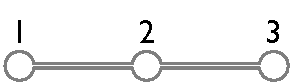
\includegraphics[width=.2\textwidth]{img/sample-1.pdf}

%If you start in hall~$2$ and visit the rest of the halls in the order $2$, $1$, $2$, $3$,
Jos aloitat salista~$2$ ja kuljet loput saleista järjestyksessä $2$, $1$, $2$, $3$,
%then you can switch off their machines at time~$0$ (in hall $2$), time~$1$ (in hall $1$), and time~$3$ (in hall $3$).
voit sammuttaa koneet ajanhetkillä $0$ (salissa $2$), $1$ (salissa $1$) ja $3$ (salissa $3$).
% This wastes $0+1+3=4$~liters of liquid in total.
Tällöin menee hukkaan yhteensä $0+1+3=4$~litraa nestettä.
% If instead you start in hall~$1$ and visit the halls in the order $1$, $2$, $3$, the total amount of liquid wasted is $0+1+2=3$~liters, which is better.
Jos sen sijaan aloitat salista~$1$ ja kuljet salit järjestyksessä $1$, $2$, $3$, nestettä menee hukkaan yhteensä vain $0+1+2=3$~litraa, mikä on parempi.

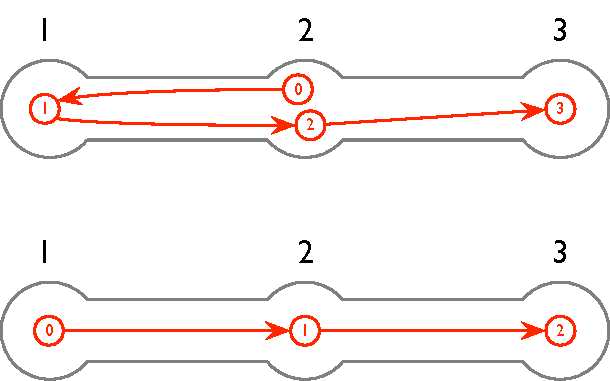
\includegraphics[width=.4\textwidth]{img/sample-1-ans.pdf}

\section*{Syöte}

%The first line of input consists of the integer $n$, denoting the number of halls.
Syötteen ensimmäisellä rivillä on yksi kokonaisluku $n$, salien määrä.
% We assume that the halls are numbered $1$, $\ldots$, $n$.
Hallit on numeroitu luvuilla $1$, $\ldots$, $n$.
% The next $n-1$ lines each contain two space-separated integers $u$ and $v$ with 
Jokainen seuraavista $n-1$ rivistä sisältää kaksi välilyönnillä erotettua kokonaislukua $u$ ja $v$, joille pätee
$1\leq u < v \leq n$, % constraint:hallnames
tarkoittaen, että salien $u$ ja $v$ välillä on tunneli.

\section*{Tuloste}

% Print a single integer: the minimum amount of spilled liquid, in liters.
Tulosta yksi kokonaisluku: pienin mahdollinen litramäärä hukkaan mennyttä nestettä.

\section*{Rajoitukset ja pisteytys}

Aina pätee
$1\leq n\leq 10^5$. % constraint:n

Ratkaisu testataan testiryhmillä, joista kullakin on oma pistemäärä.
Jokainen testiryhmä sisältää joukon testitapauksia.
Ryhmän pisteet saa vain, jos ratkaisee kaikki sen testitapaukset.
Tehtävän lopullinen pistemäärä on suurin yksittäisen lähetyksen pistemäärä.

\medskip
\begin{tabular}{lll}
Ryhmä & Pisteet & Rajoitukset \\\hline
  $1$ & $18$ & mistään salista ei lähde yli kahta tunnelia \\
  $2$ & $19$ & enintään yhdestä salista lähtee yli kaksi tunnelia \\
  $3$ & $20$ & $n\leq 10$\\
  $4$ & $21$ & $n\leq 1000$\\
  $5$ & $22$ & \emph{Ei muita rajoituksia}
\end{tabular}
